\chapter{Snow Wetness Estimation Using Dual Polarimetric SAR Data}
\section{Introduction}
High topographic mountain regions have great physical diversity with the environment. Particularly, the snow cover and its seasonal changes play an important role. The snow wetness in the Himalayan snowpack is an important parameter for snow-melt runoff modeling, snow avalanche risk assessment, climatology, hydro-power industry and weather forecasting. Satellite remote sensing is a key tool in monitoring the snow pack parameters over a large area. Microwave remote sensing measurements can be efficiently used to infer bulk properties of snowpack. In comparison to conventional single-channel Synthetic Aperture Radar (SAR), the introduction of SAR polarimetry can significantly improve the quality of the results.
These improvements are due to the quantitative ability of polarimetric SAR to scattering mechanisms. Hence, remote sensing using polarimetric SAR data has great potential in determining the extent and the properties of snow cover.

Shi $\emph{et al.}$ developed an inversion model to estimate snow wetness using SAR data based on the first-order scattering model considering both surface and volume scattering~\cite{Shi93}. The NASA/JPL airborne AIRSAR imaging polarimetric data was used in this study. However, the first-order scattering model do not apply for most natural surfaces as they are very rough on the radar wavelength scale. The Integral Equation Model (IEM) which is valid over a wider range of surface roughness is used for the inversion model to estimate snow wetness~\cite{Shi95}. The polarimetric space-borne Shuttle Imaging Radar Mission C-band (SIR-C) data was used for this study. The above method was modified to estimate snow wetness from conventional dual-polarization ENVISAT-ASAR data~\cite{Singh2010}. Statistical inversion model was also developed to retrieve snow wetness using ENVISAT-ASAR alternating polarization data~\cite{niang2007new}.

In this chapter a snow wetness estimation method for dual-polarimetric coherent (HH/VV) SAR data (\emph{i.e.,} TerraSAR-X) is proposed which is based on the work of~\cite{jagdhuber2013polarimetric} for soilmositure. The dominant surface and volume scatterings for the wet snow lead us to estimate the snow surface and snowpack volume wetness. The snow surface wetness is estimated by using the simplified IEM model for high frequency limit of X-band (9.6 GHz) data. The snow volume wetness is estimated under the Rayleigh scattering assumption. The proposed method is used to estimate the snow wetness of the top layers of the snowpack. The results obtained from the proposed method are validated with the near real time in-situ measurements with the satellite pass.

\section{Study Area and Data Used}
The field campaign was conducted to collect the in-situ measurements synchronized with the TerraSAR-X data acquisition on 23 January 2009 (the area outline in blue in Fig.~\ref{fig:study_area_dual_pol}). Along with this dataset, three more TerraSAR-X datasets acquired on 12 January 2009, 18 January 2009 and 24 January 2009 (the area outlined as red in Fig.~\ref{fig:study_area_dual_pol}) have also been used to infer the snow wetness changes over the study area. The Solang observatory where the field campaign was conducted is marked (green star) in Fig.~\ref{fig:study_area_dual_pol}. The date, time of acquisition, pass and incidence angles of the data used in this study are given in Table~\ref{table:data acquisition_sw_dual}.
\begin{table}[!htbp]
	\caption{Data Acquisition Table}
	\begin{center}
		\begin{tabular}{| c | c |c | c |c |} \hline
			No & Date & Acq. Time (IST) & Pass & Inc. Angle ($^\circ$) \\ \hline \hline
			1 & 12 Jan 2009 & 6:14 AM & Des & 38.3-39.4\\ \hline
			2 & 18 Jan 2009 & 6:24 PM & Asc & 47.3-48.2\\ \hline
			3 & 23 Jan 2009 & 6:24 AM & Des & 38.1-39.1\\ \hline
			4 & 24 Jan 2009 & 6:15 PM & Asc & 32.1-33.3\\ \hline
		\end{tabular}
	\end{center}
	\label{table:data acquisition_sw_dual}
\end{table}
The in-situ snow wetness was measured with a dielectric moisture meter~\cite{denoth1989snow,denoth1995electron}. The snow probe was used for measuring the permittivity, $\varepsilon$ of the snow medium. The volumetric liquid water content $W(\mbox{Vol}\%)$ was calculated from the measured snow permittivity, $\varepsilon$ and the snow density, $\rho$, using the following empirical relation~\cite{denoth1995electron}:
\begin{equation}
W(\mbox{Vol}\%)=5.35\left[\varepsilon-(1+1.92\rho)\right]
\label{eq:denoth}
\end{equation}
\begin{figure}[!htbp]
	\centering
	\includegraphics[width=\columnwidth]{Figures/study_area_sw_dual}
	\caption{Study area along with the footprints of the TerraSAR-X acquisitions. The Solang observatory is indicated by a green star in the image.}
	\label{fig:study_area_dual_pol}
\end{figure}
\section{Methodology}
%\newcounter{MYtempeqncnt2}
%The dual-polarimetric coherent TerraSAR-X data can be represented by a 2x2 coherency matrix ([$T_2$]) given in ~\ref{eq:coherency_matrix_dual}. In this study we will analyze this coherency matrix to estimate the snow surface and the snow volume wetness. 
%\begin{equation}
%\begin{split}
%\resizebox{0.9\columnwidth}{!}{
%	$
%	\left[T_2\right]= \frac{1}{2} \left[ \begin{array}{ccc}
%	<|S_{HH}+S_{VV}|^2> & <(S_{HH}+S_{VV})(S_{HH}-S_{VV}^*)>\\
%	<(S_{HH}+S_{VV})(S_{HH}+S_{VV}^*)> & <|S_{HH}-S_{VV}|^2>\\
%	\end{array}\right]
%	$
%}
%\label{eq:coherency_matrix_dual}
%\end{split}
%\end{equation}
%In order to estimate the snow surface wetness, the simplified IEM scattering model is used to obtain the dominant scattering magnitude $(\alpha_1)$ under the high frequency limit of X-band (9.6 GHz)~\cite{allain2003}. The IEM model has been shown to be valid for a wide range of surface roughness~\cite{Fung92,fung1994microwave}. Usually a wet snow surface is rougher than a dry snow surface because of selective melting and re-freezing.  
%
%A snow layer is an inhomogeneous medium composed of scattering elements such as ice particles and water inclusions of different shapes, sizes, and orientations~\cite{Shi95}. At a given sensor frequency, the snow density and the liquid water content affect the permittivity of snow. For the study of snow volume wetness, the Rayleigh scattering assumption has been used, where the particles of the medium are considered substantially smaller than the incident wavelength. Finally, the effective snow wetness is obtained by suitably weighing the surface and the volume snow wetness components. The weights are obtained from the eigen-decomposition of the [$T_2$] matrix.
%% %Reframe the paragraph
%
%The in-situ measurements were obtained synchronously with the TerraSAR-X pass in January. Snow wetness measurements were taken at every 5 cm depth of the standing snow. The average wetness measurement is considered as the effective snow wetness which is then used to validate the results obtained from the proposed method.
%
%\subsection{Snow Surface Wetness}
%The dominant polarimetric scattering angle $(\alpha_1)$, corresponding to the dominant eigenvector and the eigenvalue is obtained from the dual coherent [$T_2$] matrix as shown in~(\ref{eq:alphas}).
%\begin{equation}
%\begin{split}
%[T_2] &= [U_2][\Sigma][U_2]^T \\
%U_2 &= \left[ \begin{array}{ccc}
%u_{11} & u_{12} \\
%u_{21} & u_{22} \\
%\end{array} \right] \\
%\alpha_1 &= \cos ^{ - 1}(|u_{11}|) 
%\end{split}
%\label{eq:alphas}
%\end{equation}
%where $[U_2]$ is a 2$\times$2 unitary matrix of the eigenvectors, $[\Sigma]$ is a 2$\times$2 diagonal matrix of the eigenvalues and the superscript $T$ denote matrix transpose. In the high frequency limit, like X-band (9.5 GHz), the dominant polarimetric scattering angle $(\alpha_1)$ obtained from the dual-polarimetric data is compared with the scattering angle $(\alpha_{IEM})$ estimated from the simplified IEM model for high frequency $(\nu)$ limit of X-band data ~(\ref{eq:highfreq})~\cite{allain2003}. 
%\begin{equation}
%\alpha_1 \approx \lim\limits_{\nu \rightarrow High}(\alpha_{IEM}) 
%\label{eq:highfreq}
%\end{equation}
%
%The estimated $(\alpha_{IEM})$ from the simplified IEM model is only a function of the local incidence angle, $\theta$ and the surface dielectric constant $(\varepsilon_s)$ and is independent of the terrain roughness~(\ref{eq:iemalpha}). The local incidence angle $(\theta)$ is obtained using an external DEM (e.g. SRTM DEM).
%\begin{equation}
%\begin{split}
%\lim\limits_{\nu \rightarrow High} (\alpha_{IEM}) &= \atan\left( \frac{2f_{hh}f_{vv}^{*}-X}{2f_{hh}f_{vv}^{*}+X}\right) \\
%X = \left|f_{vv}\right|^2 - \left|f_{hh}\right|^2 + &\sqrt{\left(\left|f_{vv}\right|^2 - \left|f_{hh}\right|^2\right)^2 + 4\left|f_{hh}f_{vv}^{*}\right|^2}
%\end{split}
%\label{eq:iemalpha}
%\end{equation}
%The $f_{hh}=-\frac{2F_{hh}}{\cos\theta}$ and $f_{vv}=\frac{2F_{vv}}{\cos\theta}$ are the co-polarization scattering coefficients, where $F_{hh}$ and $F_{vv}$ are the Fresnel reflection coefficient for each polarization as a function of the local incidence angle $(\theta)$ and the dielectric constant $(\varepsilon_s)$.
%This estimated surface dielectric constant $(\varepsilon_s)$ is then used to compute the snow surface wetness using the Denoth's method $(W_s (\rho_d,\varepsilon_s))~\eqref{eq:denoth}~$~\cite{denoth1995electron}, where $\rho_d$ is the dry snow density.
%
%\subsection{Snow Volume Wetness}
%Apart from the snow surface wetness component, a small amount of snow volume wetness component is also expected with X-band data from a standing snow cover over ground since the penetration depth of the probing wave will be limited. The volume scattering of the snowpack is modeled as a random volume in this study. The snowpack particle structure shows high spatial variation and as a result of which it is difficult to model its volume scattering component. In this context, the particle anisotropy has been used to account for all snow particle structures. The anisotropy parameter which is interpreted in terms of the particle geometry is also characterized by the ratio of principal values of polarizability~\cite{cloude2009polarisation}. A random volume scattering coherency matrix is used in this study~(\ref{eq:volumemodel}) where $f_v$ is the volume scattering intensity and $A$ represents the particle anisotropy. 
%\begin{equation}
%\begin{split}
%\frac{f_v}{(1+A^2)} \left[ \begin{array}{cc}
%V_{11} & V_{12} \\
%V_{12}^* & V_{22} \\
%\end{array} \right]= \left[ \begin{array}{cc}
%\frac{1}{2} & 0 \\
%0 & \frac{1}{4} \\ 
%\end{array} \right] \\
%V_{11} = \frac{1}{2} (A+1)^2 ; V_{12} = 0 ;
%V_{22} =\frac{1}{4}(A-1)^2 \\
%\end{split}
%\label{eq:volumemodel}
%\end{equation}
%
%The volume scattering intensity ($f_v$) is a function of the cross-polarization component ($S_{xx}$) in quad-polarimetric case. But, unlike in the quad-polarimetric data, the cross-polarization component is unavailable in the dual-polarimetric X-band $(\mbox{HH/VV})$ coherent data. Hence, this cross-polarization component is synthesized from the dual-polarimetric data under the azimuthally symmetric condition~(\ref{eq:crosspolestimation}).  
%\begin{equation}
%\begin{split}
%f_v &= 8<|S_{xx}|^2> \\
%<|S_{xx}|^2> &= \frac{1}{4} \left(1-\gamma_{HHVV}\right)\left(<|S_{HH}|^2>+<|S_{VV}|^2>\right) \\
%\gamma_{HHVV} &= \frac{<S_{HH}S^*_{VV}>}{\sqrt{<|S_{HH}|^2><|S_{VV}|^2>}}
%\end{split}
%\label{eq:crosspolestimation}
%\end{equation}
%The quality of the estimated cross-polarization component cannot be assessed in this study due to the unavailability of a quad-polarimetric TerraSAR-X data along with the dual-polarimetric (HH/VV) coherent data. However, it has been shown that the Root Mean Square Error (RMSE) of the synthesized cross-polarization component for the TerraSAR-X data is around 1.8-2.0 dB compared to 5.0-5.4 dB for L-band E-SAR data over agricultural areas~\cite{Jagdhuber2014}. In this work our study area is a snow cover over flat bare ground devoid of any vegetation for which the condition of azimuthal symmetry can be assumed to be valid. By solving for the particle anisotropy $(A)$, it can be readily seen that it is a function of the volume scattering intensity $(f_v)$. In general the anisotropy parameter which is an indicator of particle shape is also bounded by the dielectric constant~(\ref{eq:anisotropy})~\cite{ablitt2000characterisation}. This dielectric constant is then used to estimate the volume snow wetness.
%\begin{figure}[!htbp]
%	% ensure that we have normalsize text
%	\normalsize
%	% Store the current equation number.
%	\setcounter{MYtempeqncnt2}{\value{equation}}
%	% Set the equation number to one less than the one
%	% desired for the first equation here.
%	% The value here will have to changed if equations
%	% are added or removed prior to the place these
%	% equations are referenced in the main text.
%	\setcounter{equation}{9}
%	\begin{equation}
%	W_e=
%	\begin{cases}
%	\bar{\lambda}_{1}W_s(\rho_p,\varepsilon_s) + \bar{\lambda}_{2}W_v(\rho_d,\varepsilon_v) \quad: W_s(\rho_p,\varepsilon_s) > W_v(\rho_d,\varepsilon_v) \\ 
%	\bar{\lambda}_{1}W_v(\rho_p,\varepsilon_s) + \bar{\lambda}_{2}W_s(\rho_d,\varepsilon_v) \quad: W_v(\rho_p,\varepsilon_s) > W_s(\rho_d,\varepsilon_v) \\
%	\end{cases}
%	\bar{\lambda}_{i} = \frac{\lambda_i}{\sum_{i=1,2}^{}\lambda_i}, \quad
%	\bar{\lambda}_{1} > \bar{\lambda}_{2}
%	\label{eq:effectivewetness}
%	\end{equation}		
%	% Restore the current equation number.
%	\setcounter{equation}{\value{MYtempeqncnt2}}
%	% IEEE uses as a separator
%	\hrulefill
%	% The spacer can be tweaked to stop underfull vboxes.
%	%\vspace*{2pt}
%\end{figure}
%\begin{equation}
%\frac{1}{\varepsilon_v} < A < \frac{\varepsilon_v + 1}{2}
%\label{eq:anisotropy}
%\end{equation}
%
%In order to have an approximate estimate of $\varepsilon_v$, we have combined the lower and the upper bounds of the inequality involving the anisotropy parameter and $\varepsilon_v$. Any estimate of  $\varepsilon_v$ cannot lie below the curve given by $1/ A$ and below the line given by $2A-1$. An estimating function for $\varepsilon_v$ satisfying both these conditions is given by~(\ref{eq:volumedielctric}). As the value of the anisotropy parameter increases from 0 to 1, there is a rapid fall in the estimate of $\varepsilon_v$ as dictated by the lower bound. At $A=1$, the lower and the upper bounds of the inequality converge, and $\varepsilon_v$ is estimated as unity. Beyond this point there is a linear rise in the estimate of $\varepsilon_v$. 
%\begin{equation}
%\varepsilon_v = \frac{1}{A} + \left| \frac{1}{A} - (2A - 1)\right|
%\label{eq:volumedielctric}
%\end{equation}
%
%Similar to the snow surface wetness estimation, the volume dielectric constant $\varepsilon_v$ is used to estimate the snow volume wetness using the Denoth's method $(W_v (\rho_d,\varepsilon_v))$~\eqref{eq:denoth}, where $\rho_d$ is the dry snow density as used before. The effective snow wetness $(W_e)$ is estimated as a weighted average of the surface and the volume snow wetness according to~(\ref{eq:effectivewetness}). The pseudo probabilities computed from the eigenvalues are used to weigh $W_s(\rho_p,\varepsilon_s)$ and $W_v(\rho_d,\varepsilon_v)$ to estimate $W_e$. In the high frequency limit for the wet snow cover condition ($W_s(\rho_p,\varepsilon_s) > W_v(\rho_d,\varepsilon_v)$), the surface scattering is mostly the dominant scattering mechanism. Owing to this criteria, the surface wetness $W_s(\rho_p,\varepsilon_s)$ is weighted with the first dominant eigenvalue, $\bar{\lambda}_{1}$ and subsequently the volume wetness $W_v(\rho_d,\varepsilon_v)$ is weighted with the second dominant eigenvalue, $\bar{\lambda}_{2}$. In some cases (fairly less), when $W_v(\rho_p,\varepsilon_s) > W_s(\rho_d,\varepsilon_v)$, the volume wetness, $W_v(\rho_d,\varepsilon_v)$ is weighted with the first dominant eigenvalue, $\bar{\lambda}_{1}$ and the surface snow wetness, $W_s(\rho_p,\varepsilon_s)$ is weighted with the second dominant eigenvalue, $\bar{\lambda}_{2}$ to calculate the effective snow wetness $W_{e}$. The flowchart of the proposed snow wetness estimation methodology is shown in Fig.~\ref{fig:flow_chart}.
%
%\begin{landscape}
%	\begin{figure}[!htbp]
%		\centering
%		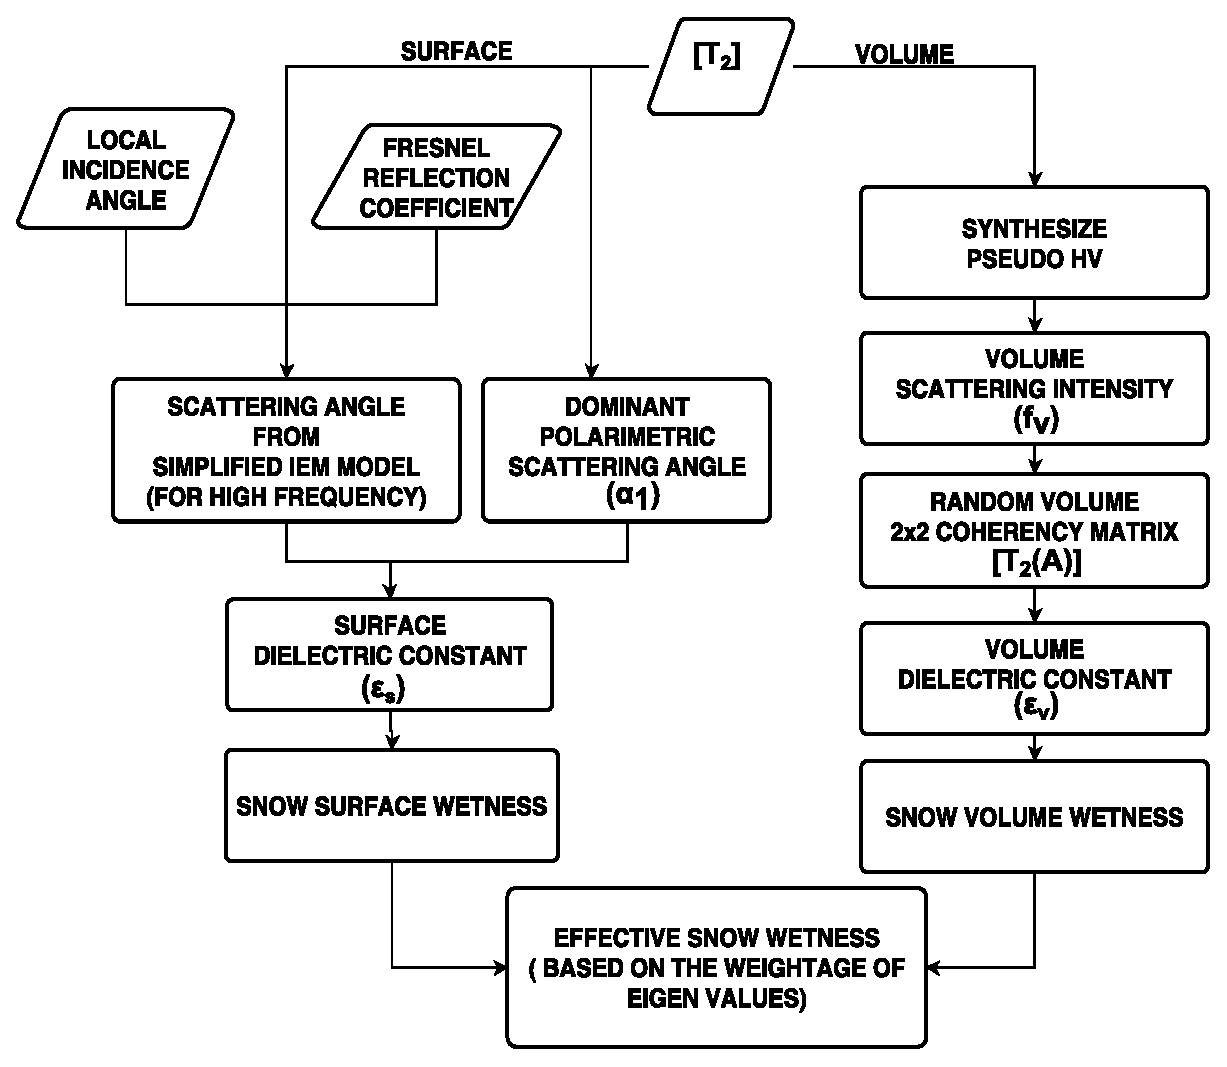
\includegraphics[width=0.8\columnwidth]{Figures_SW2/flow_chart}
%		\caption [Flowchart of snow wetness estimation method for dual-pol data]{Flowchart of the proposed snow wetness estimation methodology}
%		\label{fig:flow_chart}
%	\end{figure}	
%\end{landscape}

%\section{Results and Discussion}
%The snow wetness map for the 23 January 2009 data estimated by the proposed method is shown in Fig.~\ref{fig:proposed_results}(c). It can be seen that major part of the study area exhibits wetness in the range of 0-6$\%$ by volume. This data was acquired in descending pass and the temperature recorded during the pass was around 2.5$^\circ$C. At some places the estimated wetness is in the range of 5-10$\%$ by volume. This could be possible due to a slight amount of rainfall (5.8 mm) over the Solang valley which is evident from the observatory data (Table~\ref{table:observatory_data}). Since the snow temperature is lower than the downpour water, the snow has absorbed the downpour water temperature and began to melt. However, there are blanks (white pixels) in the right hand side of the wetness map. This could be because of geometric distortions (possibly shadow) due to a slope facing away from the radar. All images with descending passes used in this study have similar blank portions. The snow wetness results estimated by the proposed method for this dataset is compared with the in-situ measurements Fig.~\ref{fig:validation_plot}. It can be seen that the estimated snow wetness by the proposed method are closer to the in-situ measurements. Except for few points most of them show good agreement with the in-situ measurements. This could be attributed to the fact that the in-situ measurements were collected during the day in which some of the measurements were asynchronous with the satellite pass. This may be the cause for variation in the comparison of the wetness values. The overall mean absolute error for the proposed method is 1.65$\%$ by volume.
%
%\begin{figure}[!htbp]
%	\centering
%	\subfloat[]{\includegraphics[width=0.5\textwidth]{Figures_SW2/12Jan}} 
%	\subfloat[]{\includegraphics[width=0.5\textwidth]{Figures_SW2/18Jan}} \\
%	\subfloat[]{\includegraphics[width=0.5\textwidth]{Figures_SW2/23Jan}}
%	\subfloat[]{\includegraphics[width=0.5\textwidth]{Figures_SW2/24Jan}}
%	\caption[Snow wetness maps for dual-pol SAR data]{Snow wetness maps for dual polarimetry data derived from the proposed method.} 
%	\label{fig:proposed_results_dualpol}
%\end{figure}
%
%\begin{figure}[!htbp]
%	\centering
%	\includegraphics[width=\columnwidth]{Figures_SW2/validation_plot_1}
%	\caption [Validation of snow wetness method for dual pol data]{Comparison of the estimated snow wetness by the proposed method with the in-situ measurements.}
%	\label{fig:validation_plot_dualpol}
%\end{figure}
%
%The proposed snow wetness estimation method is also applied to three other TerraSAR-X datasets acquired during the same season (12, 18 and 24 January 2009). The snow wetness map for 12 Jan shows low values (0-2$\%$) for most of the study area as shown in Fig.~\ref{fig:proposed_results_dualpol}(a) which could be due to very low temperature (-3.5$^\circ$C) during the acquisition (descending). On 18 January, there was a snow fall of 13 cm and the maximum temperature recorded for the day (FN and AN) was 4$^\circ$C (Table~\ref{table:observatory_data}). These conditions are reflected in Fig.~\ref{fig:proposed_results_dualpol}(b), where most of the area is covered with dry snow. On 24 January, the standing snow has reduced by 7 cm within a span of less than 12 hours with the temperature varying from 4.0 - 10.5$^\circ$C (Table~\ref{table:observatory_data}). The snow wetness is observed to vary from 3-10$\%$ as seen in Fig.~\ref{fig:proposed_results_dualpol}(d) due to this temperature variation.
%\begin{table}[t]
%	\caption [Observatory data during dual-pol SAR data acquisitions]{Observatory Data}
%	\begin{center}
%		\begin{tabular}{| c | c | c | p{1.5cm} | p{1.5cm} | p{1.5cm} | c |} \hline
%			No & Date  & FN /AN  & Max Temp ($^\circ$C)  & Min Temp ($^\circ$C)  & Rain fall (mm)  & Standing Snow (cm)\\ \hline \hline
%			1 & 12 Jan 2009 & F  &      & -3.5 &-  & 22\\ \hline
%			2 & 12 Jan 2009 & A  & 14.5 &      &-  & 18\\ \hline 
%			3 & 18 Jan 2009 & F  &      & 1.0  &-  & 7\\ \hline
%			4 & 18 Jan 2009 & A  &  4   &      &-  & 20\\ \hline 
%			5 & 19 Jan 2009 & F  &      & -0.5 &-  & 26\\ \hline
%			6 & 19 Jan 2009 & A  &  11  &      &-  & 17\\ \hline 
%			7 & 20 Jan 2009 & F  &      & -1.5 &-  & 17\\ \hline
%			8 & 20 Jan 2009 & A  &  15  &      &-  & 15\\ \hline 
%			9 & 21 Jan 2009 & F  &      & 1.5  &-  & 15\\ \hline
%			10 & 21 Jan 2009 & A &  16  &      &-  & 12\\ \hline 
%			11 & 22 Jan 2009 & F &      & 1.5  &-  & 12\\ \hline
%			12 & 22 Jan 2009 & A &  6   &      &-  & 12\\ \hline 
%			13 & 23 Jan 2009 & F &      & 2.5  & 5.8 & 10\\ \hline
%			14 & 23 Jan 2009 & A &  12  &      &-  & 12\\ \hline 
%			15 & 24 Jan 2009 & F &      & 4.0  &-  & 12\\ \hline
%			16 & 24 Jan 2009 & A &  10.5&      &- & 5\\ \hline 
%		\end{tabular}
%	\end{center}
%	\label{table:observatory_data}
%\end{table}
%
%\section{Conclusion}
%In this chapter, we have proposed a new methodology for snow wetness estimation from dual-~polarimetric (HH/VV) coherent high frequency (9.6 GHz) SAR data. In this high frequency limit, the snow surface and the volume scattering components are considered to estimate the snow wetness. The surface wetness is derived from the simplified IEM model whereas the volume wetness is derived using the Rayleigh scattering assumption. The proposed methodology is applied to four TerraSAR-X datasets over the Indian Himalayan region. However, the validation has been carried out only for 23 Jan 2009 dataset, as the synchronous ground measurements were available only for this day. The overall mean absolute error for the proposed method is 1.65$\%$ by volume. It can also be seen that for 12, 18 and 24 January 2009 datasets the proposed method is able to correctly estimate the snow wetness for varying weather conditions. The proposed method is suitable for flat areas without vegetation cover, which can be further modified to account for the same. 